% !TeX root = document.tex
\chapter{Maschinelle Werteanpassung}

Es ist schwer menschliche Werte in Computersystemen zu programmieren (siehe Kapitel \ref{Werte}), deshalb haben \citeauthor{irving_ai_2018} einen anderen Ansatz der Werteanpassung verfolgt: die des menschlichen Feedbacks durch \emph{Deep reinforcement learning} (DRL, dt. \emph{mehrschichtiges bestärkendes Lernen}; siehe Abbildung \ref{humanfeedbackimg}). Das folgende Unterkapitel dient der Erklärung von wichtigen Lernverfahren der KI-Forschung, um die wissenschaftlichen Arbeiten von \citeauthor{irving_ai_2018} zu verstehen.

\section{KI-Lernverfahren}
\subsection{Reinforcement Learning}
Reinforcement Learning (RL, dt. \emph{bestärkendes Lernen}) beschreibt ein Lernverfahren einer KI, bei der sie durch durch Erfolg und Misserfolg, durch Belohnung und Bestrafung lernt. \citeauthor{russell_artificial_2016} erklären RL zusammengefasst so: \zit[831]{russell_artificial_2016}{Imagine playing a new game whose rules you don't know; after a hundred or so moves, your opponent announces, \enquote{You lose.} This is reinforcement learning in a nutshell.}

Die Aufgabe von RL ist es, wahrgenommene Belohnungen und Bestrafungen zu benutzen, um die optimale Verfahrensweise (eng. \emph{policy}) in einer gegebenen Umgebung zu finden. Dabei hat die KI a priori kein Wissen über ihre Umgebung oder Nutzfunktion. Die Nutzfunktion, definiert über Umgebungszustände, zeigt dabei den Nutzen einer bestimmten Verfahrensweise. Die optimale Verfahrensweise ist diejenige, die den höchsten erwarteten Nutzen bringt.

RL wird in Bereichen eingesetzt, in denen es nicht genug Daten gibt, oder in denen es nicht lohnenswert ist, die notwendige Menge an Daten zu verarbeiten, um eine KI auf alle möglichen Umgebungszustände vorzubereiten. Eine KI, die beispielsweise versucht, Schach zu lernen, müsste $10^{120}$ (auch Shannon-Zahl genannt) verschiedene Schachspiele gesehen haben, um allein anhand von Beispielen auf jede Situation vorbereitet zu sein. \vgl[4]{shannon_programming_1988} Bei RL vermittelt man der KI stattdessen, wann sie gewonnen oder verloren hat. Sie sucht dann auf Basis dieser Informationen eine Funktion, die die Gewinnwahrscheinlichkeit jeder gegebenen Position einigermaßen akkurat einschätzt.
\vgl[830-831]{russell_artificial_2016}

\subsection{Deep Learning}
Deep Learning (DL, dt. \emph{mehrschichtiges Lernen}) ist ein Teilbereich des maschinellen Lernens. Dabei versucht eine KI Inputdaten mit Hilfe von Hierarchien von Konzepten zu verstehen. Der Grundansatz von DL ist das Verstehen von komplexen Konzepten durch Kombinieren von einfacheren Konzepten (siehe Abbildung \ref{deeplearningimg}). Diese Konzeptschichten werden in DL fast immer mit Hilfe von künstlichen neuronalen Netzen (KNN, engl. \emph{artificial neural network, ANN}) gelernt. \vgl[8]{chollet_deep_2017} Die Anzahl der Schichten wird auch Tiefe (eng. \emph{depth}) genannt, daher der Name Deep Learning.
\vgl[1-8]{Goodfellow-et-al-2016}

DL wird heute vor allem in den Bereichen der Sprach- und Bilderkennung sowie der maschinellen Übersetzung eingesetzt. \vgl[25-26]{Goodfellow-et-al-2016}

\begin{figure}
  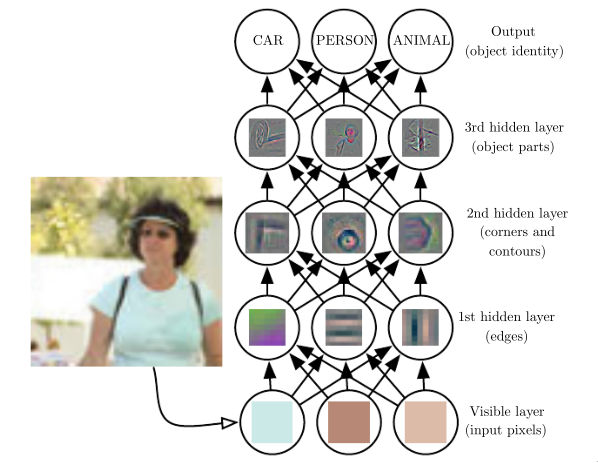
\includegraphics[width=\textwidth]{deeplearning}
  \caption{Veranschaulichung eines DL-Modells. Die KI bekommt rohe Pixeldaten als Input. Mit jeder Schicht wendet sie ein neues Konzept auf das vorherige an, die Konzepte sind also aufbauend. Durch Analyse der Helligkeit umgebener Pixeln werden Ränder erkannt (1. Schicht). Ansammlungen von Rändern werden als Ecken und Konturen identifiziert (2. Schicht). Durch zusammenhängende Ecken und Konturen können ganze Objektteile bestimmt werden (3. Schicht).  \bildquelle[6]{Goodfellow-et-al-2016}}
  \label{deeplearningimg}
\end{figure}
\subsection{Deep Reinforcement Learning}

Deep Reinforcement Learning (DRL, dt. \emph{mehrschichtiges bestärkendes Lernen}) kombiniert die Ansätze von RL mit denen von DL. Neuronale Netze werden trainiert, um jeder möglichen Aktion in einer gegebenen Umgebungsposition einen Nutzwert zuzuteilen. Ihr Ziel ist es, die nützlichste Aktion zu finden. \vgl{nicholson_beginners_nodate} Auf der Abbildung \ref{deepreinforcementlearningimg} wird dieser Vorgang mit einem Frame des Spiels \emph{Mario Bros.} als Input veranschaulicht. Diese Nutzwertzuteilung ermöglicht eine signifikante Leistungsteigerung von RL in bestimmten Domänen.

\citeauthor{mnih_human-level_2015} haben einen Algorithmus entwickelt, mit dem eine KI allein anhand von Pixeln als Input gelernt hat, 49 verschiedene \emph{Atari 2600} Spiele zu spielen, 29 davon sogar auf menschenähnlichem Niveau. \vgl{mnih_human-level_2015}



\begin{figure}
  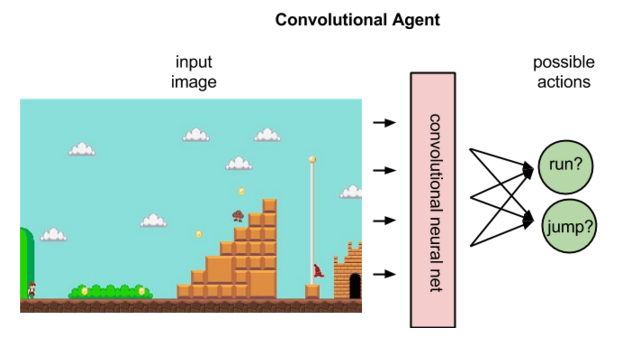
\includegraphics[width=\textwidth]{deepreinforcementlearning}
  \caption{Die Umgebung ist das Level, in dem sich Mario (links unten zu sehen) befindet, die möglichen Aktionen sind: springen, nach links laufen, nach rechts laufen. Die neuronalen Netze teilen jeder Aktion einen Nutzwert zu. Beispiel: springen (5), nach rechts laufen (7), nach links laufen (0). \bildquelle{nicholson_beginners_nodate}}
  \label{deepreinforcementlearningimg}
\end{figure}

\subsection{Inverse Reinforcement Learning}
Inverse Reinforcement Learning (IRL, dt. \emph{umgekehrtes bestärkendes Lernen}) ist ein Lernverfahren, bei dem eine KI versucht anhand von Input-Output-Paaren die richtige Lösungsfunktion herzuleiten. Dies ist in allen Bereichen sinnvoll, in denen man (noch) nicht weiß, was das Ziel ist oder in denen es schwer ist, das gewollte Verhalten formell in eine Nutzfunktion auszuschreiben. Ein solcher Fall ist das autonome Fahren. Ein angenehmer und sicherer Fahrstil hängt abgesehen von den Verkehrsregeln noch mit vielen anderen Faktoren zusammen: der Sicherheitsabstand, der Bremsstil, die ökonomische Fahrweise, das Spurhalten, das Rechtsfahren, der Abstand vom Randstein, eine angemessene Fahrgeschwindigkeit oder die Anzahl an Spurwechseln um einige zu nennen. Alle relevanten Faktoren müssten formell ausgeschrieben und gewichtet werden, damit das System weiß, dass der Abstand zu Fußgängern beispielsweise wichtiger ist als der Abstand zum Randstein. Nur so kann ein autonomes Fahrzeug im Zweifelsfall die richtigen Entscheidungen treffen. Statt alle relevanten Faktoren auszuformulieren und zu gewichten, zeigt man einer KI Beispiele von angenehmen und sicheren Fahrstilen und lässt die KI die Nutz- und die Lösungsfunktion herleiten und anpassen. \vgl{abbeel_apprenticeship_2004} Nachdem eine Lösungsfunktion gefunden wurde, kann diese durch RL trainiert werden. \vgl[1]{christiano_deep_2017}


\section{Deep Reinforcement Learning von menschlichen Werten}
Die größte Sorge der KI-Forschung ist, dass wir Zielfunktionen unzureichend definieren und eine KI dadurch Schaden anrichtet, mit anderen Worten: dass eine KI nicht das tut, was wir \enquote{meinen} (siehe Kapitel \ref{bösartigeKI}).\vgl[1]{yudkowsky_complex_2011} IRL löst dieses Problem, da die Zielfunktion von der KI selbst definiert wird. Der Ansatz funktioniert aber nur bei Aufgaben, für die es auch Lösungsdemonstrationen gibt. Eine Alternative ist, das Verhalten des Systems zu gegebenen Zeitpunkten von Menschen beurteilen zu lassen. \citeauthor{christiano_deep_2017} haben eine KI im ersten Schritt ihre Nutzfunktion durch menschliches Feedback lernen lassen. Im zweiten Schritt optimiert die KI ihre Nutzfunktion, sie versucht sich also so zu verhalten, dass der menschliche Begutachter möglichst zufriedengestellt ist. So handelt die KI nach den menschlichen Werten und ihre Ziele stimmen mit den unseren überein. Diese beiden Schritte werden so lange wiederholt, bis die KI das gewünschte Verhalten zeigt (siehe Abbildung \ref{humanfeedbackimg}). \vgl[1-2]{christiano_deep_2017} Es folgt eine formelle Ausformulierung.

Zu jedem Zeitpunkt $t$ empfängt die KI eine Umgebungsobservation $o_t \in \mathcal{O}$ und sendet dann eine Aktion $a_t \in \mathcal{A}$ an die Umgebung. Wir nehmen an, dass ein menschlicher Begutachter seine Präferenz zwischen Trajektoriensegmenten auswählt, wobei ein Trajektoriensegment eine Abfolge von Observationen und Aktionen ist: $\sigma = ((o_0,a_0),(o_1,a_1),...,(o_{k-1},a_{k-1})) \in (\mathcal{O} \times \mathcal{A})^k$. Man schreibt $\sigma^1 \succ \sigma^2$, um auszudrücken, dass der Begutachter das Trajektoriensegment $\sigma^1$ über dem Segment $\sigma^2$ bevorzugt. \vgl[3-4]{christiano_deep_2017}

In den Experimenten von \citeauthor{christiano_deep_2017} bekommt der menschliche Begutachter Trajektoriensegmente in Form von ein- bis zweisekündigen Videoclips zugespielt. Die Begutachtung kommt in eine Datenbank $\mathcal{D}$ bestehend aus dreidimensionalen Arrays ($\sigma^1,\sigma^2,\mu$), wobei $\mu$ eine Distribution über $\{1,2\}$ ist.

\begin{enumerate}
\item Falls eines der Segmente bevorzugt wird, dann wird die jeweilige Auswahl mehr gewichtet.
\item Falls der Begutachter beide als gleich wünschenswert erachtet, so ist $\mu$ eine Konstante.
\item Falls die Segmente als nicht vergleichbar eingestuft werden, dann wird der jeweilige Vergleich aus der Datenbank $\mathcal{D}$ exkludiert.
\vgl[5]{christiano_deep_2017}
\end{enumerate}
  
Weiters stellen \citeauthor{christiano_deep_2017} eine Formel zur Berechnung der Wahrscheinlichkeit $\hat{P}$ auf, dass ein Begutachter das Trajektoriensegment $\sigma^1$ bevorzugt.
\begin{equation}
  \hat{P}[\sigma^1 \succ \sigma^2] = \frac{exp \sum \hat{r} (o_t^1,a_t^1)}{exp \sum \hat{r}(o^1_t,a^1_t) + exp \sum \hat{r}(o^2_t, a^2_t)}
\end{equation}

$\hat{r}$ ist eine Belohnungsfunktion, also eine Funktion, die die Wahrscheinlichkeit angibt, dass die Trajektorie $(o^1,a^1)$ zum Zeitpunkt $t$ zu einer Belohnung führt. Die Summe der Belohnungsfunktionen zu allen Zeitpunkten $t$ ergibt die gesamte erwartete Belohnung für das Trajektoriensegment $\sigma^1$. Der Quotient von der Gesamtbelohnung von $\sigma^1$ und der Summe der Gesamtbelohnungen beider Segmente ergibt $\hat{P}$. Man bemerke, dass die Autoren alle Summen der Gleichung exponieren. Das liegt daran, dass die Belohnungswahrscheinlichkeit mit zunehmender Zeit exponentiell steigt. Genauso wie der Elopunkten-Unterschied zwischen verschiedenen Schachspielern in etwa die Wahrscheinlichkeit angibt, dass einer gegen den anderen gewinnt, zeigt der Unterschied des erwarteten Gewinns zweier Trajektoriensegmente in etwa die Wahrscheinlichkeit, dass eines vom Begutachter präferiert wird.
\vgl[5]{christiano_deep_2017}

\begin{figure}
  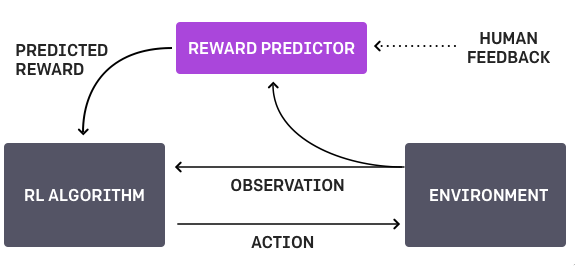
\includegraphics[width=\textwidth]{humanfeedback}
  \caption{Repräsentation einer human-feedback-loop \bildquelle{amodei_learning_2017}}
  \label{humanfeedbackimg}
\end{figure}

\section{KI-Sicherheit durch KI-Debatten}
DRL von menschlichen Werten ist ein funktionierender Ansatz, damit eine (A)KI die komplexen Werte und Ziele der Menschheit erkennt und sich ihnen ausrichtet. Er funktioniert aber nur so lange, bis der Begutachter nicht mehr in der Lage ist, das Handeln der KI nachzuvollziehen und zu beurteilen. \vgl[1-2]{irving_ai_2018}



% Hierbei fragt eine KI einen menschlichen Operator nach der Nützlichkeit und Sicherheit ihres Verhaltens. Bei schlechter Bewertung passt die KI ihre Lösungsfunktion an, somit ist weder eine Werteprogrammierung, noch eine riskante Zielsetzung im Vorhinein notwendig. \vgl{christiano_deep_2017} Dies funktioniert so lange gut, bis der Operator nicht mehr in der Lage ist, das Handeln der KI nachzuvollziehen und zu beurteilen. \vgl[1-2]{irving_ai_2018}
\section{AI Safety via Debate}
\section{Inverse Reward Design}

%Was ist eine Reward function?
%Eine Nutzfunktion ist 


%Ein Algorithmus einer sicheren AKI muss die folgenden Probleme lösen:
%\begin{enumerate}
%\item Negative Effekte durch eine fehlerhaft definierte Nutzfunktion zur Feststellung der Ziele
%\item Eine AKI könnte eine Problemstellung mit der Intention, sie wieder lösen zu können, verschlimmern. (Ein Staubsaugroboter, der Staub herstellt, um ihn dann wieder aufsaugen zu können.) \vgl[1-2]{hadfield-menell_inverse_2017}
%\end{enumerate}

%https://80000hours.org/articles/ai-safety-syllabus/
%\vgl{yudkowsky_intelligence_2013}
%\section{Wertekodierung in einer Programmiersprache}
%KOMMENTAR: Complexity of Value Theory
%\subsection{Statische Wertekodierung}
%\subsection{Dynamisch-maschinelle Werteanpassung}
%
%\section{Mensch-Maschinen-Interface}
%\section{Hirnemulation}
%\section{Friendly AI}



%%% Local Variables:
%%% mode: latex
%%% TeX-master: "document"
%%% End:
